% Made up for the tikra benchmark.
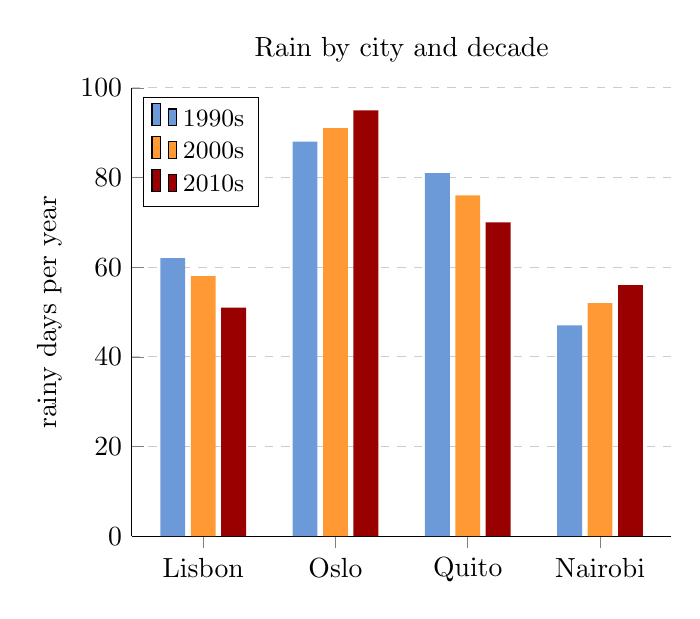
\begin{tikzpicture}
\begin{axis}[ybar, bar width=9pt, ymin=0, ymax=100, enlarge x limits=0.18,
    symbolic x coords={Lisbon, Oslo, Quito, Nairobi}, xtick=data,
    ylabel={rainy days per year}, title={Rain by city and decade},
    legend style={at={(0.02,0.98)}, anchor=north west, font=\small},
    ymajorgrids, grid style={dashed, gray!40}, axis x line*=bottom, axis y line*=left]
  \addplot[fill=cyan!50!blue!60, draw=none] coordinates {(Lisbon,62) (Oslo,88) (Quito,81) (Nairobi,47)};
  \addplot[fill=orange!80, draw=none] coordinates {(Lisbon,58) (Oslo,91) (Quito,76) (Nairobi,52)};
  \addplot[fill=red!60!black, draw=none] coordinates {(Lisbon,51) (Oslo,95) (Quito,70) (Nairobi,56)};
  \legend{1990s, 2000s, 2010s}
\end{axis}
\end{tikzpicture}
